\documentclass[multi=tikzpicture, border=0pt]{standalone}
\usepackage{tikz}
\usepackage{graphicx}

\begin{document}
\begin{tikzpicture}
  % Image size: 4.5cm wide, ~3.22cm tall (729x521 px aspect ratio)
  \pgfmathsetmacro{\iw}{4.5}
  \pgfmathsetmacro{\ih}{4.5 * 521 / 729}
  \pgfmathsetmacro{\gap}{0.02}
  \pgfmathsetmacro{\colB}{\iw + \gap}
  \pgfmathsetmacro{\colC}{2*(\iw + \gap)}
  \pgfmathsetmacro{\rowA}{2*(\ih + \gap)}
  \pgfmathsetmacro{\rowB}{\ih + \gap}

  % ── Row 1: sp | F | F ──
  \node[anchor=south west, inner sep=0] at (0, \rowA)
    {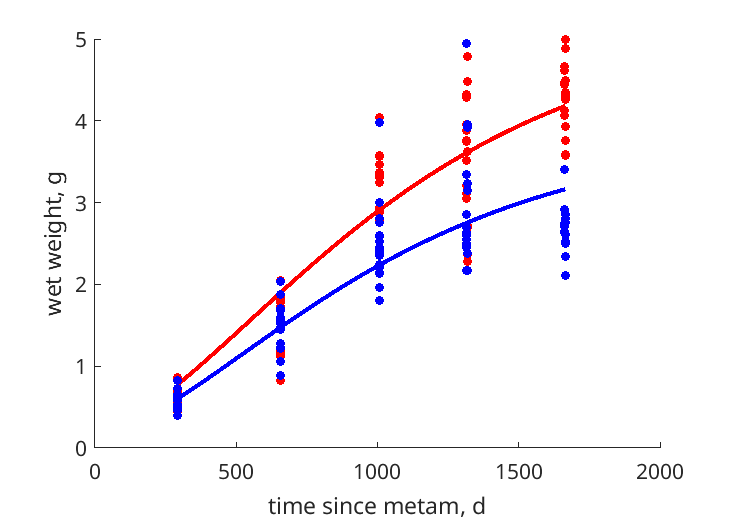
\includegraphics[width=\iw cm]{../../sp/results_Ichthyosaura_alpestris_02.png}};
  \node[anchor=north west, inner sep=2, fill=white, fill opacity=0.7, text opacity=1] at (0.7, \rowA+\ih-0.1) {\scriptsize Population-average};

  \node[anchor=south west, inner sep=0] at (\colB, \rowA)
    {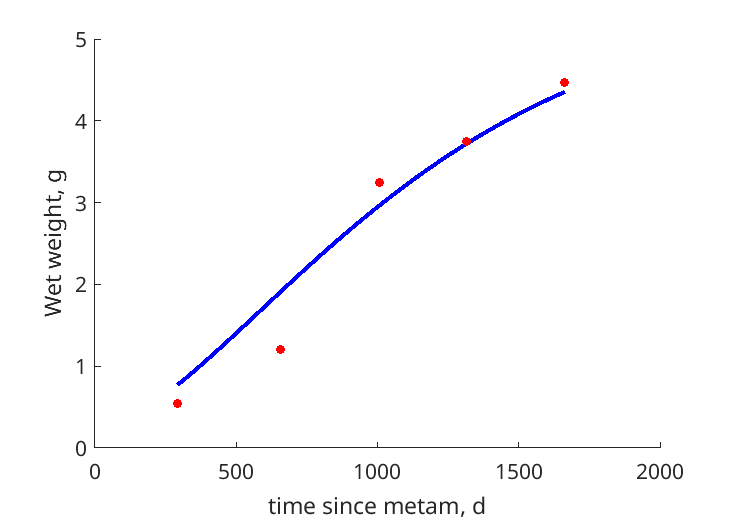
\includegraphics[width=\iw cm]{../../ind/8045/results_Ichthyosaura_alpestris_02.png}};
  \node[anchor=north west, inner sep=2, fill=white, fill opacity=0.7, text opacity=1] at (\colB+0.7, \rowA+\ih-0.1) {\scriptsize Female 8045};

  \node[anchor=south west, inner sep=0] at (\colC, \rowA)
    {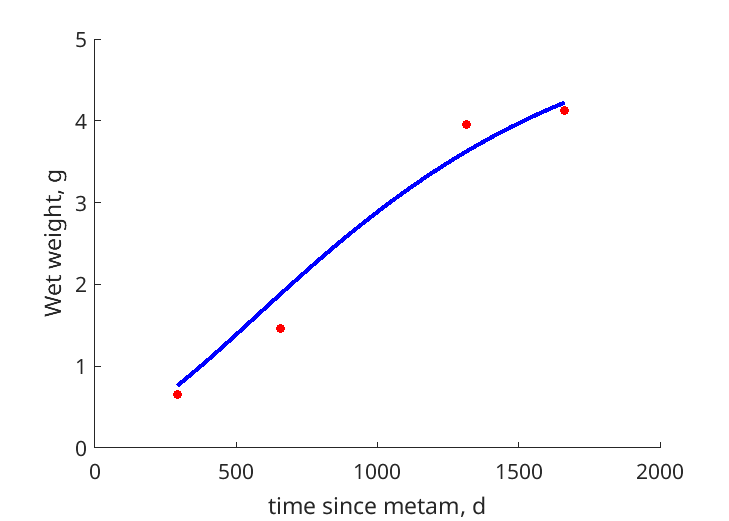
\includegraphics[width=\iw cm]{../../ind/8050/results_Ichthyosaura_alpestris_02.png}};
  \node[anchor=north west, inner sep=2, fill=white, fill opacity=0.7, text opacity=1] at (\colC+0.7, \rowA+\ih-0.1) {\scriptsize Female 8050};

  % ── Row 2: F | F | M ──
  \node[anchor=south west, inner sep=0] at (0, \rowB)
    {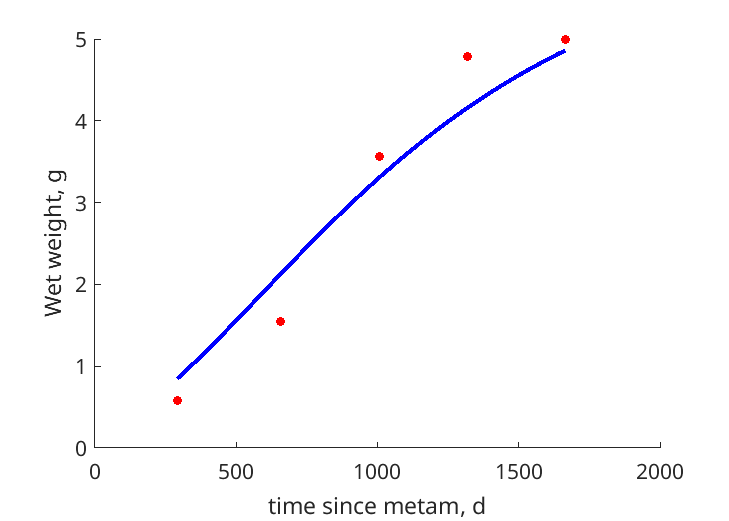
\includegraphics[width=\iw cm]{../../ind/8069/results_Ichthyosaura_alpestris_02.png}};
  \node[anchor=north west, inner sep=2, fill=white, fill opacity=0.7, text opacity=1] at (0.7, \rowB+\ih-0.1) {\scriptsize Female 8069};

  \node[anchor=south west, inner sep=0] at (\colB, \rowB)
    {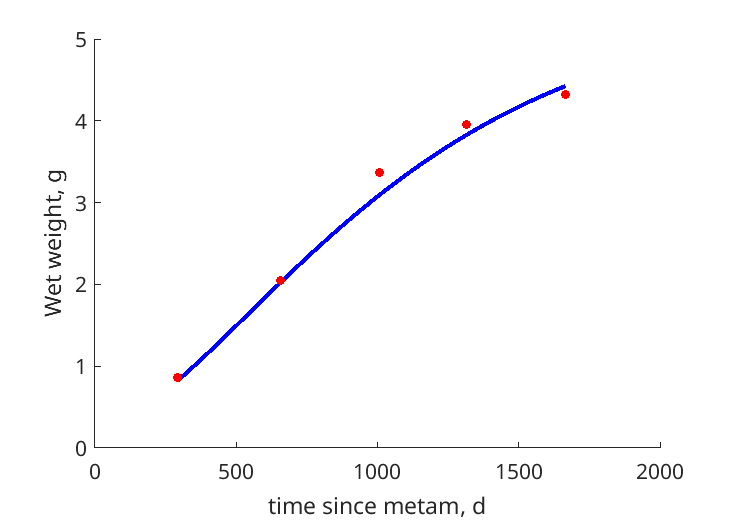
\includegraphics[width=\iw cm]{../../ind/8078/results_Ichthyosaura_alpestris_02.png}};
  \node[anchor=north west, inner sep=2, fill=white, fill opacity=0.7, text opacity=1] at (\colB+0.7, \rowB+\ih-0.1) {\scriptsize Female 8078};

  \node[anchor=south west, inner sep=0] at (\colC, \rowB)
    {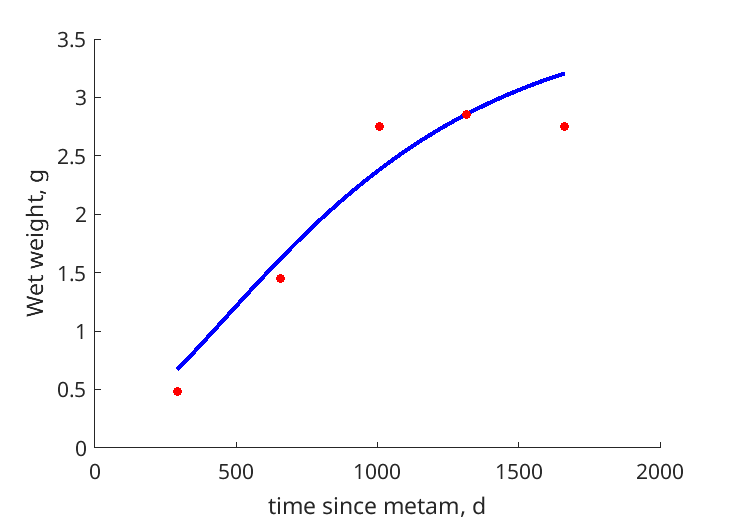
\includegraphics[width=\iw cm]{../../ind/8046/results_Ichthyosaura_alpestris_02.png}};
  \node[anchor=north west, inner sep=2, fill=white, fill opacity=0.7, text opacity=1] at (\colC+0.7, \rowB+\ih-0.1) {\scriptsize Male 8046};

  % ── Row 3: M | M | M ──
  \node[anchor=south west, inner sep=0] at (0, 0)
    {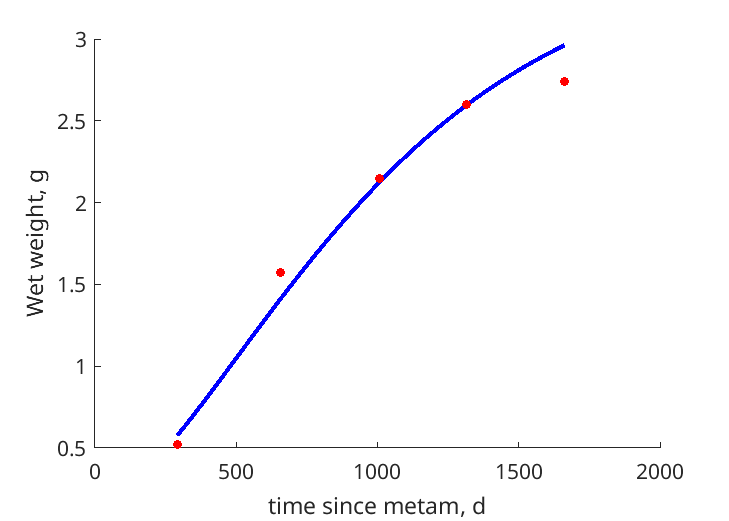
\includegraphics[width=\iw cm]{../../ind/8053/results_Ichthyosaura_alpestris_02.png}};
  \node[anchor=north west, inner sep=2, fill=white, fill opacity=0.7, text opacity=1] at (0.7, \ih-0.1) {\scriptsize Male 8053};

  \node[anchor=south west, inner sep=0] at (\colB, 0)
    {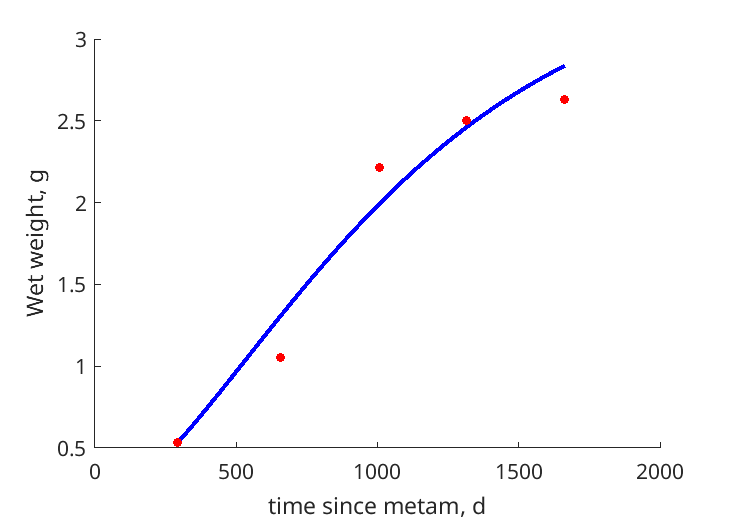
\includegraphics[width=\iw cm]{../../ind/8058/results_Ichthyosaura_alpestris_02.png}};
  \node[anchor=north west, inner sep=2, fill=white, fill opacity=0.7, text opacity=1] at (\colB+0.7, \ih-0.1) {\scriptsize Male 8058};

  \node[anchor=south west, inner sep=0] at (\colC, 0)
    {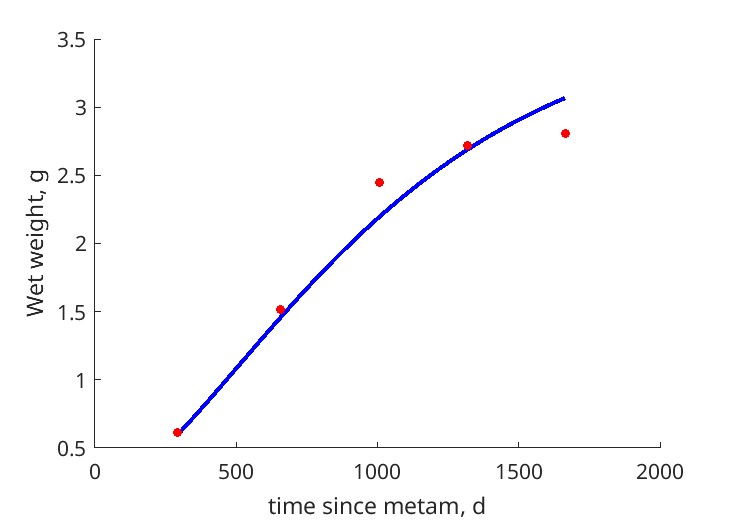
\includegraphics[width=\iw cm]{../../ind/8073/results_Ichthyosaura_alpestris_02.png}};
  \node[anchor=north west, inner sep=2, fill=white, fill opacity=0.7, text opacity=1] at (\colC+0.7, \ih-0.1) {\scriptsize Male 8073};
\end{tikzpicture}
\end{document}
